\documentclass[xcolor=table,      handout ,    xcolor=dvipsnames]{beamer}\usepackage[]{graphicx}\usepackage[]{color}
% maxwidth is the original width if it is less than linewidth
% otherwise use linewidth (to make sure the graphics do not exceed the margin)
\makeatletter
\def\maxwidth{ %
  \ifdim\Gin@nat@width>\linewidth
    \linewidth
  \else
    \Gin@nat@width
  \fi
}
\makeatother


\definecolor{fgcolor}{rgb}{0, 0, 0}
\newcommand{\hlnum}[1]{\textcolor[rgb]{0,0,0}{#1}}
\newcommand{\hlstr}[1]{\textcolor[rgb]{0.545,0.137,0.137}{#1}}
\newcommand{\hlcom}[1]{\textcolor[rgb]{0,0.392,0}{\textit{#1}}}
\newcommand{\hlopt}[1]{\textcolor[rgb]{0,0,0}{#1}}
\newcommand{\hlstd}[1]{\textcolor[rgb]{0,0,0}{#1}}
\newcommand{\hlkwa}[1]{\textcolor[rgb]{1,0,0}{\textbf{#1}}}
\newcommand{\hlkwb}[1]{\textcolor[rgb]{0,0,0}{#1}}
\newcommand{\hlkwc}[1]{\textcolor[rgb]{1,0,1}{#1}}
\newcommand{\hlkwd}[1]{\textcolor[rgb]{0,0,1}{#1}}


\usepackage{framed}
\makeatletter
\newenvironment{kframe}{%
 \def\at@end@of@kframe{}%
 \ifinner\ifhmode%
  \def\at@end@of@kframe{\end{minipage}}%
  \begin{minipage}{\columnwidth}%
 \fi\fi%
 \def\FrameCommand##1{\hskip\@totalleftmargin \hskip-\fboxsep
 \colorbox{shadecolor}{##1}\hskip-\fboxsep
     % There is no \\@totalrightmargin, so:
     \hskip-\linewidth \hskip-\@totalleftmargin \hskip\columnwidth}%
 \MakeFramed {\advance\hsize-\width
   \@totalleftmargin\z@ \linewidth\hsize
   \@setminipage}}%
 {\par\unskip\endMakeFramed%
 \at@end@of@kframe}
\makeatother

\definecolor{shadecolor}{rgb}{.97, .97, .97}
\definecolor{messagecolor}{rgb}{0, 0, 0}
\definecolor{warningcolor}{rgb}{1, 0, 1}
\definecolor{errorcolor}{rgb}{1, 0, 0}
\newenvironment{knitrout}{}{} % an empty environment to be redefined in TeX

\usepackage{alltt} % , handout, draft
\usetheme{Madrid} % Madrid, Warsaw, Berlin
\usecolortheme{beaver}

\usepackage[latin1]{inputenc} % windows
%\usepackage[utf8]{inputenc} %linux
\usepackage[T1]{fontenc} % for textbackslash
\usepackage[german, english]{babel}
\usepackage{float} % placing floats (table and figures) where they should be
\usepackage{lmodern} % make tiny font shape warnings within the beamer class diappear
\usepackage{tabu, multirow, url, hyperref, textcomp, amsmath, listings, datetime, graphicx, booktabs, xcolor, multicol, setspace}
\usepackage[absolute,overlay,showboxes]{textpos}
\usepackage{wasysym}
\usepackage{fontawesome}

\hypersetup{pdfstartview={XYZ null null 1}}
\hypersetup{colorlinks=true, linkcolor=blue, urlcolor=blue}

\setbeamertemplate{footline}[text line]{%
  \parbox{\linewidth}{\vspace*{-8pt}
  \href{https://github.com/brry/course\#slides}{github.com/brry/course} \hfill
  \hyperlink{toc}{TOC} ~~ \insertframenumber / \inserttotalframenumber~~~~~~~~~}}
\setbeamertemplate{navigation symbols}[only frame symbol]

\beamersetleftmargin{0.3cm}
\beamersetrightmargin{0.3cm}

% Reduce spacing in table of contents (toc) http://tex.stackexchange.com/questions/51452
\usepackage{etoolbox}
\makeatletter
\patchcmd{\beamer@sectionintoc}{\vskip1.5em}{\vskip0.1em}{}{} % vskip0.5em
\makeatother

% Remove Bullets and Numbers in TOC: http://tex.stackexchange.com/questions/54656
\setbeamertemplate{sections/subsections in toc}[default]

% white letters in enumerate bullet points
%\definecolor{stupidblue}{RGB}{51,51,178}
\setbeamercolor{item projected}{fg=white}%fg=blue,bg=red!75!black} % fg=white , bg=stupidblue
\setbeamercolor{frametitle}{fg=black}
% Block title color
\setbeamercolor{block title}{fg=white}%fg=blue,bg=red!75!black} % white
%\setbeamertemplate{item projected}[square]


% define an environment for the exercises
\newcounter{exercisecount}
\setcounter{exercisecount}{0}
\newenvironment{exercise}[1]
{% This is the begin code
\stepcounter{exercisecount}
\begin{block}{Exercise \arabic{exercisecount}: #1}
}
{% This is the end code
\end{block} }

\resetcounteronoverlays{exercisecount}

% format inline R command names in blue courier and lightgrey background:
\newcommand{\rcode}[1]{\texttt{\textcolor{Blue}{#1}}}
\newcommand{\key}[1]{\colorbox{gray!30}{\texttt{\textcolor{Blue}{#1}}}}


% links to files
\newcommand{\datalinkRaw}[1]{\href{https://raw.githubusercontent.com/brry/course/master/data/#1}{#1}}
\newcommand{\datalinkBlob}[1]{\href{https://github.com/brry/course/blob/master/data/#1}{#1}}
\newcommand{\datalinkText}[1]{\href{https://github.com/brry/course/blob/master/data/#1}{#1} 
                            {\footnotesize \textit{(rightclick \textbf{Raw}, save as)}}}
                           
% Format month with leading zero:
\newcommand{\leadingzero}[1]{\ifnum #1<10 0\the#1\else\the#1\fi}

% "#' " for doc files:
\newcommand{\doc}{\#\textquotesingle~}

% remove empty lines between code and output. apparently hard to get rid of without turning off syntax highlighting


%------------------------------------------------------------%
%------------------------------------------------------------%
\IfFileExists{upquote.sty}{\usepackage{upquote}}{}
\begin{document}
%------------------------------------------------------------%
%------------------------------------------------------------%

\AtBeginSection[]
{
\begin{frame}%[shrink]
{Outline}
\scriptsize
\tableofcontents[sectionstyle=show/shaded, subsectionstyle=show/shaded/hide]
\end{frame}
}

%\def\newblock{}	% beamer---natbib bugfix






{\usebackgroundtemplate{
\includegraphics[width=\paperwidth]{fig/slidebg-1.pdf}}
\begin{frame}
\begin{center}
    \begin{columns}
    \column{15em}
    \begin{block}{}{\Large ~loops and functions in 
\includegraphics[width=0.7cm]{externalfig/Rlogo.png}}
    \end{block}
    \end{columns}
\vspace{1em}
Berry Boessenkool, \texttt{berry-b@gmx.de}\\
Jannes Breier, \texttt{jbreier@gfz-potsdam.de}\\[1em]
\href{https://gitext.gfz-potsdam.de/swc-bb/swc-lessons/2019-11-26-potsdam-berlin/R/tree/master/_episodes_rmd/data}{https://bit.ly/37AYX1D}\\[1em]
These slides and tasks are a subset of Berry's teaching material at\\
\href{https://github.com/brry/course}{github.com/brry/course}\\[1em]
These slides are licenced under
\href{https://creativecommons.org/licenses/by/4.0}{
\includegraphics[width=3em]{externalfig/ccby.png}},\\
so you can use the material freely as long as you cite us.\\[1em]
R installation instructions: \href{https://github.com/brry/course\#install}{github.com/brry/course\#install}\\[2em]
\scriptsize
PDF created on \the\year-\leadingzero{\month}-\leadingzero{\day}, \currenttime\ \\[1em]
\end{center}
\end{frame}
}

%------------------------------------------------------------%

\begin{frame}{Outline}
%%%\hspace{0.9em} \hyperlink{titlepage}{R course Info}\\[0.4em]
\tableofcontents[hideallsubsections]
\label{toc}
\end{frame}

%------------------------------------------------------------%

\begin{frame}{\rcode{print("Hello world!")}}
\begin{itemize}[<+->]
\item Berry Boessenkool $\rightarrow$ Geoecology @ Potsdam University
\item R Fan\onslide<+->atic \onslide<+-> since 2010
\item Developer of \href{https://github.com/brry/rdwd\#rdwd}{\texttt{rdwd}},
 \onslide<+-> Freelance trainer \& consultant \href{https://brry.github.io}{
\includegraphics[width=0.5cm]{externalfig/Blogo.png}}\\[2em]
\item Jannes Breier $\rightarrow$ Geoecology @ Potsdam University
\item Berry taught me R in 2013 \smiley{}
\item \href{https://www.linkedin.com/in/jbreier/}{\faLinkedinSquare} Research Software Engineer at GFZ, \href{https://www.gfz-potsdam.de/en/staff/jannes-breier/sec44/}{
\includegraphics[width=0.65cm]{externalfig/GFZ.png}} Sec.4.4: Hydrology \\[2em]
\item \alert{If we're proceeding too fast, please interrupt!}
\end{itemize}
\end{frame}

%------------------------------------------------------------%
%------------------------------------------------------------%
\section{For loops}
%------------------------------------------------------------%
%------------------------------------------------------------%

\begin{frame}[fragile]{For loops}
Execute a block of code several times, with different input values.\\
Syntax: ~ \texttt{\alert{for}(aRunningVariable \alert{in} aSequence)\{ doSomething \}}
\pause
Often, i (for index) is used, thus ~~ \texttt{\alert{for}(i \alert{in} 1:n) \rcode{doThis}(i)}
\pause
\begin{knitrout}
\definecolor{shadecolor}{rgb}{0.961, 0.961, 0.961}\color{fgcolor}\begin{kframe}
\begin{alltt}
\hlkwd{help}\hlstd{(}\hlstr{"for"}\hlstd{)} \hlcom{# needs quotation marks!}
\end{alltt}
\end{kframe}
\end{knitrout}
\pause
\begin{knitrout}
\definecolor{shadecolor}{rgb}{0.961, 0.961, 0.961}\color{fgcolor}\begin{kframe}
\begin{alltt}
\hlkwd{print}\hlstd{(}\hlnum{1}\hlopt{:}\hlnum{2}\hlstd{)}
\hlkwd{print}\hlstd{(}\hlnum{1}\hlopt{:}\hlnum{5}\hlstd{)}
\hlkwd{print}\hlstd{(}\hlnum{1}\hlopt{:}\hlnum{9}\hlstd{)}
\end{alltt}
\end{kframe}
\end{knitrout}
\pause
This is easier and less prone to human errors with:
\pause
\begin{knitrout}
\definecolor{shadecolor}{rgb}{0.961, 0.961, 0.961}\color{fgcolor}\begin{kframe}
\begin{alltt}
\hlkwa{for}\hlstd{(i} \hlkwa{in} \hlkwd{c}\hlstd{(}\hlnum{2}\hlstd{,}\hlnum{5}\hlstd{,}\hlnum{9}\hlstd{) ) \{} \hlkwd{print}\hlstd{(}\hlnum{1}\hlopt{:}\hlstd{i) \}}
\end{alltt}
\begin{verbatim}
## [1] 1 2
## [1] 1 2 3 4 5
## [1] 1 2 3 4 5 6 7 8 9
\end{verbatim}
\end{kframe}
\end{knitrout}
\end{frame}


%------------------------------------------------------------%

\begin{frame}[fragile]{For loops: fill a vector}
\begin{knitrout}
\definecolor{shadecolor}{rgb}{0.961, 0.961, 0.961}\color{fgcolor}\begin{kframe}
\begin{alltt}
\hlstd{v} \hlkwb{<-} \hlkwd{vector}\hlstd{(}\hlkwc{mode}\hlstd{=}\hlstr{"numeric"}\hlstd{,} \hlkwc{length}\hlstd{=}\hlnum{20}\hlstd{)}
\hlstd{v}
\end{alltt}
\begin{verbatim}
##  [1] 0 0 0 0 0 0 0 0 0 0 0 0 0 0 0 0 0 0 0 0
\end{verbatim}
\end{kframe}
\end{knitrout}
\pause \vspace{-1em}
\begin{knitrout}
\definecolor{shadecolor}{rgb}{0.961, 0.961, 0.961}\color{fgcolor}\begin{kframe}
\begin{alltt}
\hlkwa{for}\hlstd{(i} \hlkwa{in} \hlnum{3}\hlopt{:}\hlnum{17}\hlstd{)  \{  v[i]} \hlkwb{<-} \hlstd{(i}\hlopt{+}\hlnum{2}\hlstd{)}\hlopt{^}\hlnum{2}  \hlstd{\}}
\end{alltt}
\end{kframe}
\end{knitrout}
\pause \vspace{-1em}
\begin{knitrout}
\definecolor{shadecolor}{rgb}{0.961, 0.961, 0.961}\color{fgcolor}\begin{kframe}
\begin{alltt}
\hlstd{v} \hlcom{# this code was executed once for each i}
\end{alltt}
\begin{verbatim}
##  [1]   0   0  25  36  49  64  81 100 121
## [10] 144 169 196 225 256 289 324 361   0
## [19]   0   0
\end{verbatim}
\end{kframe}
\end{knitrout}
\pause \vspace{-0.5em}
In R, \rcode{for} loops are slow. Always try to vectorize (the best option, not always possible) or use \rcode{lapply} (saves you the initiation of the empty vector, easier to parallize).
\end{frame}

%------------------------------------------------------------%

\begin{frame}[fragile]{For loops: execute code multiple times I}
\hspace{5em} $y = f(x, n) = \frac{12.5*n}{(n-1)!}*(\frac{n x}{8})^{(n-1)}*e^{-\frac{n x}{8}}$
\begin{knitrout}\footnotesize
\definecolor{shadecolor}{rgb}{0.961, 0.961, 0.961}\color{fgcolor}

{\centering 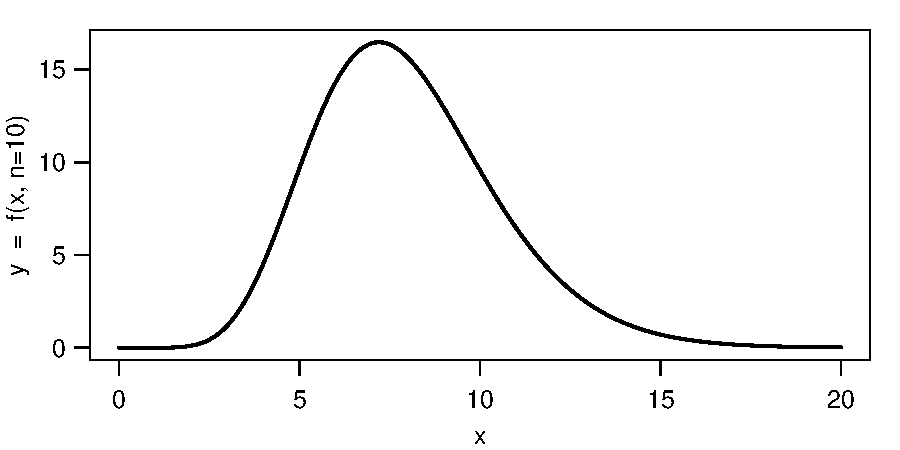
\includegraphics[width=\textwidth]{./fig/for3a-1} 

}



\end{knitrout}

\end{frame}

%------------------------------------------------------------%

\begin{frame}[fragile]{For loops: execute code multiple times II}
\textblockrulecolour{red}
\begin{knitrout}\footnotesize
\definecolor{shadecolor}{rgb}{0.961, 0.961, 0.961}\color{fgcolor}\begin{kframe}
\begin{alltt}
\hlstd{x} \hlkwb{<-} \hlkwd{seq}\hlstd{(}\hlnum{0}\hlstd{,}\hlnum{25}\hlstd{,}\hlnum{0.1}\hlstd{)}
\hlkwd{plot}\hlstd{(x,x,} \hlkwc{type}\hlstd{=}\hlstr{"n"}\hlstd{,} \hlkwc{ylab}\hlstd{=}\hlstr{"y = f(x,n)"}\hlstd{)}
\hlkwd{lines}\hlstd{(x,} \hlnum{12.5}\hlopt{*}\hlnum{5}\hlopt{/}\hlkwd{factorial}\hlstd{(}\hlnum{5}\hlopt{-}\hlnum{1}\hlstd{)}\hlopt{*}\hlstd{(x}\hlopt{/}\hlnum{8}\hlopt{*}\hlnum{5}\hlstd{)}\hlopt{^}\hlstd{(}\hlnum{5}\hlopt{-}\hlnum{1}\hlstd{)}\hlopt{*}\hlkwd{exp}\hlstd{(}\hlopt{-}\hlstd{x}\hlopt{/}\hlnum{8}\hlopt{*}\hlnum{5}\hlstd{),} \hlkwc{col}\hlstd{=}\hlnum{2}\hlstd{)}
\hlkwd{lines}\hlstd{(x,} \hlnum{12.5}\hlopt{*}\hlnum{6}\hlopt{/}\hlkwd{factorial}\hlstd{(}\hlnum{6}\hlopt{-}\hlnum{1}\hlstd{)}\hlopt{*}\hlstd{(x}\hlopt{/}\hlnum{8}\hlopt{*}\hlnum{6}\hlstd{)}\hlopt{^}\hlstd{(}\hlnum{6}\hlopt{-}\hlnum{1}\hlstd{)}\hlopt{*}\hlkwd{exp}\hlstd{(}\hlopt{-}\hlstd{x}\hlopt{/}\hlnum{8}\hlopt{*}\hlnum{6}\hlstd{),} \hlkwc{col}\hlstd{=}\hlnum{2}\hlstd{)}
\end{alltt}
\end{kframe}

{\centering 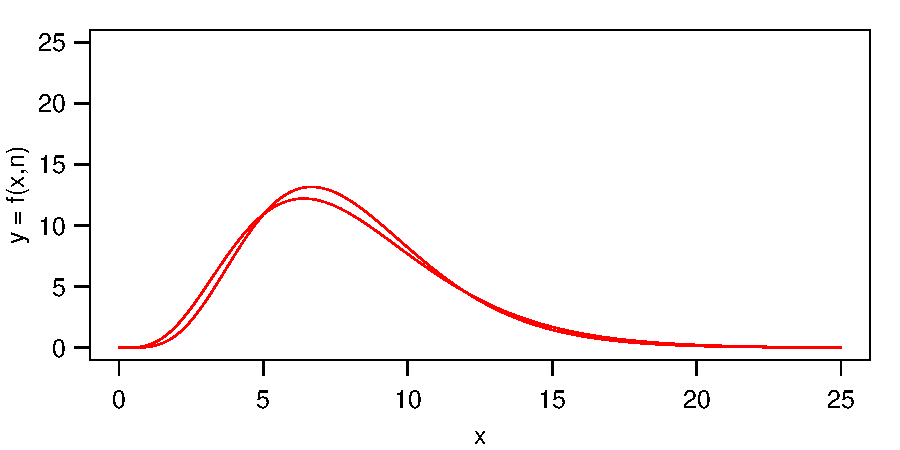
\includegraphics[width=\textwidth]{./fig/for3-1} 

}



\end{knitrout}
\only<2>{
\begin{textblock*}{0.2cm}(2.6cm,2.2cm)
\vspace{0.9cm} ~
\end{textblock*}
%
\begin{textblock*}{0.2cm}(4.6cm,2.2cm)
\vspace{0.9cm} ~
\end{textblock*}
%
\begin{textblock*}{0.2cm}(6.27cm,2.2cm)
\vspace{0.9cm} ~
\end{textblock*}
%
\begin{textblock*}{0.2cm}(6.93cm,2.2cm)
\vspace{0.9cm} ~
\end{textblock*}
%
\begin{textblock*}{0.2cm}(9.25cm,2.2cm)
\vspace{0.9cm} ~
\end{textblock*}
%
}
\end{frame}

%------------------------------------------------------------%

\begin{frame}[fragile]{For loops: execute code multiple times III}
\begin{knitrout}\footnotesize
\definecolor{shadecolor}{rgb}{0.961, 0.961, 0.961}\color{fgcolor}\begin{kframe}
\begin{alltt}
\hlstd{x} \hlkwb{<-} \hlkwd{seq}\hlstd{(}\hlnum{0}\hlstd{,}\hlnum{25}\hlstd{,}\hlnum{0.1}\hlstd{)}
\hlkwd{plot}\hlstd{(x,x,} \hlkwc{type}\hlstd{=}\hlstr{"n"}\hlstd{,} \hlkwc{ylab}\hlstd{=}\hlstr{"y = f(x,n)"}\hlstd{)}
\hlkwa{for} \hlstd{(n} \hlkwa{in} \hlnum{5}\hlopt{:}\hlnum{25}\hlstd{)}
\hlkwd{lines}\hlstd{(x,} \hlnum{12.5}\hlopt{*}\hlstd{n}\hlopt{/}\hlkwd{factorial}\hlstd{(n}\hlopt{-}\hlnum{1}\hlstd{)}\hlopt{*}\hlstd{(x}\hlopt{/}\hlnum{8}\hlopt{*}\hlstd{n)}\hlopt{^}\hlstd{(n}\hlopt{-}\hlnum{1}\hlstd{)}\hlopt{*}\hlkwd{exp}\hlstd{(}\hlopt{-}\hlstd{x}\hlopt{/}\hlnum{8}\hlopt{*}\hlstd{n),} \hlkwc{col}\hlstd{=}\hlnum{2}\hlstd{)}
\end{alltt}
\end{kframe}

{\centering 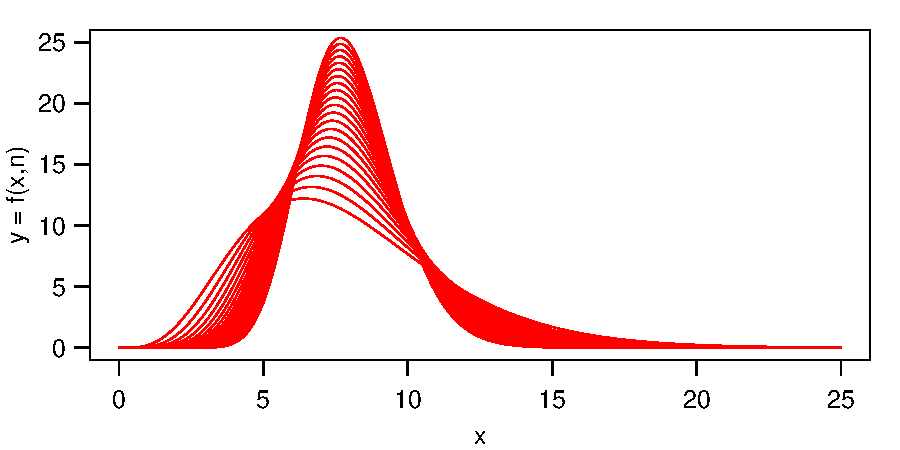
\includegraphics[width=\textwidth]{./fig/for5-1} 

}



\end{knitrout}
\begin{textblock*}{0.2cm}(2.6cm,2.65cm)
\vspace{0.45cm} ~
\end{textblock*}
%
\begin{textblock*}{0.2cm}(4.6cm,2.65cm)
\vspace{0.45cm} ~
\end{textblock*}
%
\begin{textblock*}{0.2cm}(6.27cm,2.65cm)
\vspace{0.45cm} ~
\end{textblock*}
%
\begin{textblock*}{0.2cm}(6.93cm,2.65cm)
\vspace{0.45cm} ~
\end{textblock*}
%
\begin{textblock*}{0.2cm}(9.25cm,2.65cm)
\vspace{0.45cm} ~
\end{textblock*}
%
\end{frame}


%------------------------------------------------------------%



%------------------------------------------------------------%

\begin{frame}[fragile]{For loops exercise}
\begin{exercise}{for loop}
\begin{enumerate}
\item Read \datalinkText{stocks.txt}, so that there are no factors in the data.frame. Use the command \rcode{read.table} and set the arguments \texttt{file}, \texttt{header} and \texttt{stringsAsFactors}
\item Change the first column type from \texttt{char} to \texttt{date} with \rcode{as.Date(yourDF\$Date)}
\item What do you get with \rcode{plot(yourDF[ ,c(1,2)])}? Make it a line graph by setting the argument \texttt{type}.
\item With a \rcode{for} loop, plot each stock time series, i.e. plot the \textit{i}th column over the first column.
\item BONUS 1: Use good annotations (\texttt{main, ylab, xlab})
\item BONUS 2: Turn y axis labels upright (\texttt{las})
\item BONUS 3: With \rcode{par(mfrow...}, set up a two by three panel plot
\end{enumerate}
\end{exercise}
\end{frame}

%------------------------------------------------------------%

\begin{frame}[fragile]{For loops exercise solution}
\vspace{-1em}
\begin{knitrout}\footnotesize
\definecolor{shadecolor}{rgb}{0.961, 0.961, 0.961}\color{fgcolor}\begin{kframe}
\begin{alltt}
\hlstd{stocks} \hlkwb{<-} \hlkwd{read.table}\hlstd{(}\hlstr{"data/stocks.txt"}\hlstd{,} \hlkwc{header}\hlstd{=T,} \hlkwc{stringsAsFactors}\hlstd{=}\hlnum{FALSE}\hlstd{)}
\hlstd{stocks}\hlopt{$}\hlstd{Date} \hlkwb{<-} \hlkwd{as.Date}\hlstd{(stocks}\hlopt{$}\hlstd{Date)}
\hlkwa{for}\hlstd{(i} \hlkwa{in} \hlnum{2}\hlopt{:}\hlnum{7}\hlstd{)} \hlkwd{plot}\hlstd{(stocks[ ,}\hlkwd{c}\hlstd{(}\hlnum{1}\hlstd{,i)],} \hlkwc{type}\hlstd{=}\hlstr{"l"}\hlstd{,} \hlkwc{main}\hlstd{=}\hlkwd{colnames}\hlstd{(stocks)[i],}
                   \hlkwc{ylab}\hlstd{=}\hlstr{"Stock value"}\hlstd{,} \hlkwc{las}\hlstd{=}\hlnum{1}\hlstd{)}
\end{alltt}
\end{kframe}

{\centering 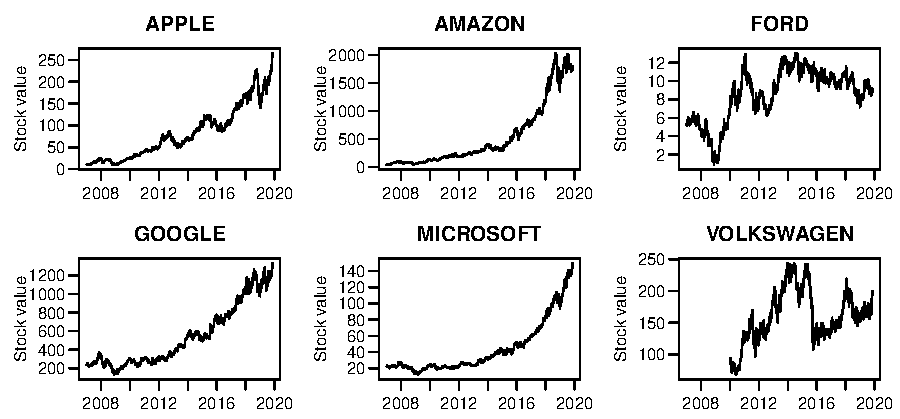
\includegraphics[width=\textwidth]{./fig/forpanel-1} 

}



\end{knitrout}
\end{frame}

%------------------------------------------------------------%

\begin{frame}[fragile]{for -> lapply}
\textbf{l}apply: apply a function to elements of a list (or vector)\\
list: R object containing other objects
\pause \vspace{-1em}
\begin{knitrout}
\definecolor{shadecolor}{rgb}{0.961, 0.961, 0.961}\color{fgcolor}\begin{kframe}
\begin{alltt}
\hlstd{files} \hlkwb{<-} \hlkwd{dir}\hlstd{(}\hlstr{"../rawdata"}\hlstd{,} \hlkwc{pattern}\hlstd{=}\hlstr{"*.csv"}\hlstd{,} \hlkwc{full}\hlstd{=}\hlnum{TRUE}\hlstd{)}
\end{alltt}
\end{kframe}
\end{knitrout}
\pause \vspace{-1em}
\begin{knitrout}
\definecolor{shadecolor}{rgb}{0.961, 0.961, 0.961}\color{fgcolor}\begin{kframe}
\begin{alltt}
\hlcom{# bad and slow way:}
\hlstd{ldfs} \hlkwb{<-} \hlkwd{list}\hlstd{()} \hlcom{# initiate empty list}
\hlkwa{for}\hlstd{(i} \hlkwa{in} \hlnum{1}\hlopt{:}\hlkwd{length}\hlstd{(files))}
   \hlstd{ldfs[[i]]} \hlkwb{<-} \hlkwd{read.csv}\hlstd{(files[i],} \hlkwc{as.is}\hlstd{=}\hlnum{TRUE}\hlstd{)}
\end{alltt}
\end{kframe}
\end{knitrout}
\pause \vspace{-1em}
\begin{knitrout}
\definecolor{shadecolor}{rgb}{0.961, 0.961, 0.961}\color{fgcolor}\begin{kframe}
\begin{alltt}
\hlcom{# much better way: apply function to each file}
\hlstd{ldfs} \hlkwb{<-} \hlkwd{lapply}\hlstd{(}\hlkwc{X}\hlstd{=files,} \hlkwc{FUN}\hlstd{=read.csv,} \hlkwc{as.is}\hlstd{=}\hlnum{TRUE}\hlstd{)}
\end{alltt}
\end{kframe}
\end{knitrout}
\pause \vspace{-1em}
\begin{knitrout}
\definecolor{shadecolor}{rgb}{0.961, 0.961, 0.961}\color{fgcolor}\begin{kframe}
\begin{alltt}
\hlcom{# progress bar with remaining time (+ parallelized!)}
\hlkwd{library}\hlstd{(}\hlstr{"pbapply"}\hlstd{)}
\hlstd{ldfs} \hlkwb{<-} \hlkwd{pblapply}\hlstd{(}\hlkwc{X}\hlstd{=files,} \hlkwc{FUN}\hlstd{=read.csv,} \hlkwc{as.is}\hlstd{=}\hlnum{TRUE}\hlstd{)}
\hlstd{ldfs} \hlkwb{<-} \hlkwd{pblapply}\hlstd{(}\hlkwc{X}\hlstd{=files,} \hlkwc{FUN}\hlstd{=read.csv,} \hlkwc{as.is}\hlstd{=}\hlnum{TRUE}\hlstd{,} \hlkwc{cl}\hlstd{=}\hlnum{8}\hlstd{)}
\end{alltt}
\end{kframe}
\end{knitrout}
\end{frame}

%------------------------------------------------------------%
%------------------------------------------------------------%
\section{Functions}
%------------------------------------------------------------%
%------------------------------------------------------------%

\begin{frame}[fragile]{Functions I}
\label{functions1}
\href{http://r4ds.had.co.nz/functions.html}{http://r4ds.had.co.nz/functions.html}\\
\pause
\rcode{?"function"}\\
\pause  Syntax:\\
\rcode{Functionobjectname <- \alert{function}(argument1, argument2, ...) \\
~~~~~~~~~~~~~~~~~~~~~~~~~~~~~~\{"DoSomething"\}}\\
\pause
\begin{knitrout}
\definecolor{shadecolor}{rgb}{0.961, 0.961, 0.961}\color{fgcolor}\begin{kframe}
\begin{alltt}
\hlstd{myfunct} \hlkwb{<-} \hlkwa{function}\hlstd{(}\hlkwc{grappig}\hlstd{)}
       \hlstd{\{}\hlkwd{plot}\hlstd{(grappig,} \hlkwc{type}\hlstd{=}\hlstr{"l"}\hlstd{);} \hlkwd{return}\hlstd{(grappig}\hlopt{*}\hlnum{7}\hlstd{)  \}}
\end{alltt}
\end{kframe}
\end{knitrout}
\pause
After \rcode{return()}ing, the execution of the function is terminated, so it should only be positioned at the end. It can also be left away, the last instruction ("expression") will then be returned.
\end{frame}

%------------------------------------------------------------%

\begin{frame}[fragile]{Functions II}
\begin{knitrout}
\definecolor{shadecolor}{rgb}{0.961, 0.961, 0.961}\color{fgcolor}\begin{kframe}
\begin{alltt}
\hlkwd{myfunct}\hlstd{(}   \hlkwd{c}\hlstd{(}\hlnum{5}\hlstd{,}\hlnum{11}\hlstd{,}\hlnum{3}\hlstd{,}\hlnum{7}\hlstd{)  )}
\end{alltt}
\begin{verbatim}
## [1] 35 77 21 49
\end{verbatim}
\end{kframe}

{\centering 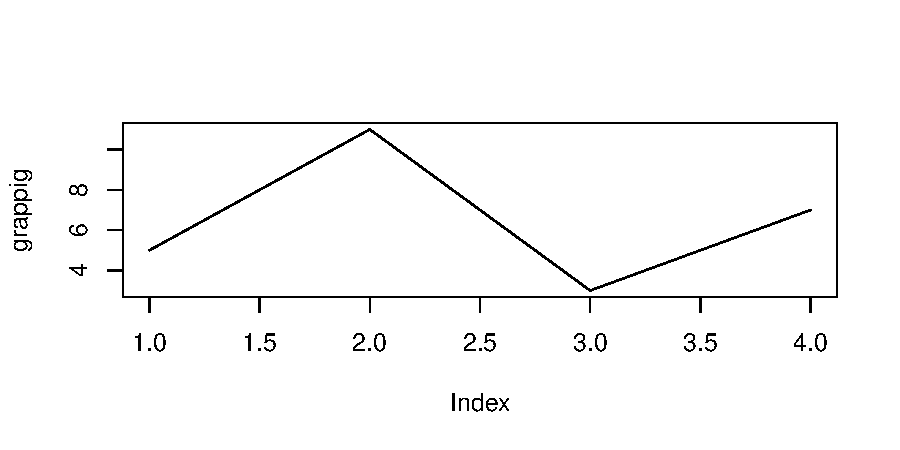
\includegraphics[width=\textwidth]{./fig/funct3-1} 

}



\end{knitrout}
\end{frame}

%------------------------------------------------------------%

\begin{frame}[fragile]{Functions with more arguments + default values}
\begin{knitrout}\small
\definecolor{shadecolor}{rgb}{0.961, 0.961, 0.961}\color{fgcolor}\begin{kframe}
\begin{alltt}
\hlstd{myfunct} \hlkwb{<-} \hlkwa{function}\hlstd{(}\hlkwc{x}\hlstd{,} \hlkwc{type}\hlstd{=}\hlstr{"b"}\hlstd{,} \hlkwc{...}\hlstd{)} \hlkwd{plot}\hlstd{(x,} \hlkwc{type}\hlstd{=type, ...)}
\hlcom{# type="b" is now the default, thus used unless specified}
\hlcom{# The ellipsis (...) passes arguments to other functions}
\hlkwd{myfunct}\hlstd{(}  \hlkwd{c}\hlstd{(}\hlnum{5}\hlstd{,}\hlnum{11}\hlstd{,}\hlnum{3}\hlstd{,}\hlnum{7}\hlstd{) ,} \hlkwc{col}\hlstd{=}\hlstr{"red"}\hlstd{,} \hlkwc{las}\hlstd{=}\hlnum{1}\hlstd{)}
\end{alltt}
\end{kframe}

{\centering 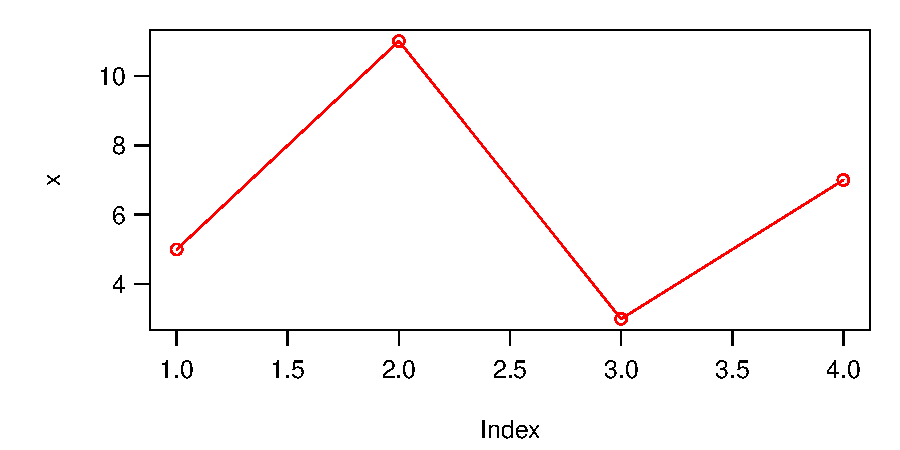
\includegraphics[width=\textwidth]{./fig/funct4-1} 

}



\end{knitrout}
\vspace{-2em}
\end{frame}

%------------------------------------------------------------%

\begin{frame}[fragile]{Conditional execution}
Syntax:
\rcode{\alert{if}(this\_is\_true) \{do\_something\}}\\
\pause
\rcode{\alert{if}(this\_is\_true) \{do\_something\} \alert{else} \{do\_other\_thing\}}\\[0.8em]
\pause
If condition == TRUE, then expression1 is evaluated,\\
if condition == FALSE, then expression2 is evaluated.\\[0.8em]
\pause
\begin{columns}
\begin{column}{.40\textwidth}
\texttt{7-3 > 2 \\
\textcolor{blue}{class}(7-3 > 2 ) \\
\textcolor{red}{if}(7-3 > 2) 18  \\
\textcolor{red}{if}(7-3 > 5) 18  \\
\textcolor{red}{if}(7-3 > 5) 18 \textcolor{red}{else} 17 }
\end{column}
\begin{column}{.59\textwidth}
\pause TRUE\\
\pause logical = truth value, boolean\\
\pause Condition is TRUE, so 18 is returned\\
\pause Condition is FALSE, so nothing happens\\
\pause Condition FALSE, so 17 is returned.
\end{column}
\end{columns}
\pause \vspace{0.8em}
\begin{knitrout}
\definecolor{shadecolor}{rgb}{0.961, 0.961, 0.961}\color{fgcolor}\begin{kframe}
\begin{alltt}
\hlkwa{if}\hlstd{(}\hlkwd{length}\hlstd{(input)}\hlopt{>}\hlnum{1}\hlstd{)}
  \hlkwd{stop}\hlstd{(}\hlstr{"length must be 1, not "}\hlstd{,} \hlkwd{length}\hlstd{(input))}
\end{alltt}
\end{kframe}
\end{knitrout}
\pause \vspace{-0.3em}
\rcode{stop}: Interrupts function execution and gives error\\
\rcode{warning}: continues but gives warning\\
\rcode{message}: to inform instead of worry the user\\[1em]
\end{frame}

%------------------------------------------------------------%

\begin{frame}[fragile]{Exercise: add circles with given radius}
\begin{knitrout}
\definecolor{shadecolor}{rgb}{0.961, 0.961, 0.961}\color{fgcolor}\begin{kframe}
\begin{alltt}
\hlkwd{plot}\hlstd{(}\hlnum{1}\hlopt{:}\hlnum{10}\hlstd{,} \hlkwc{asp}\hlstd{=}\hlnum{1}\hlstd{)} \hlcom{# aspect ratio y/x of graph range}
\hlkwd{grid}\hlstd{(}\hlkwc{col}\hlstd{=}\hlnum{1}\hlstd{)}
\hlcom{# the next part sould go into a function:}
\hlstd{x} \hlkwb{<-} \hlnum{8} \hlstd{;  y} \hlkwb{<-} \hlnum{6} \hlstd{;  r} \hlkwb{<-}\hlnum{2}
\hlstd{p} \hlkwb{<-} \hlkwd{seq}\hlstd{(}\hlnum{0}\hlstd{,} \hlnum{2}\hlopt{*}\hlstd{pi,} \hlkwc{len}\hlstd{=}\hlnum{50}\hlstd{)}
\hlstd{cx} \hlkwb{<-} \hlstd{x}\hlopt{+}\hlstd{r}\hlopt{*}\hlkwd{cos}\hlstd{(p) ;  cy} \hlkwb{<-} \hlstd{y}\hlopt{+}\hlstd{r}\hlopt{*}\hlkwd{sin}\hlstd{(p)}
\hlkwd{polygon}\hlstd{(cx, cy)}
\end{alltt}
\end{kframe}

{\centering 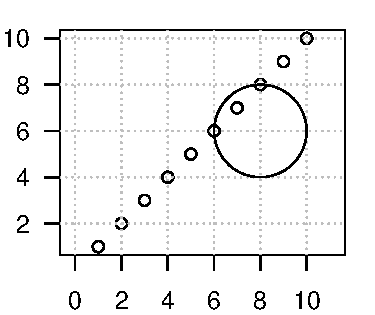
\includegraphics[width=0.4\textwidth]{./fig/circlebasics-1} 

}



\end{knitrout}
\end{frame}

%------------------------------------------------------------%

\begin{frame}[fragile]{Time to practice programming}
\begin{exercise}{Writing functions} %ex
Write a function that
\begin{enumerate}
  \item - draws a circle with a certain radius at user-specified locations of an existing plot (see last slide).
  \item - uses ellipsis (\rcode{...}) to allow the user to customize the appearance
  \item - checks all the arguments and gives useful warnings if the wrong type of input is provided
  \item - has useful explanations for each argument (documentation)
  \item - has readable indentation, spacing and comments explaining the code
  \item Now let your neighbor use it without explaining how it is to be used (this should be inferred from the code and comments!)
  \item Use your neighbor's function with a vector to draw several circles at once. (unintended use?) What happens?
  \item BONUS: Learn writing packages at \datalinkText{packdev.R}
\end{enumerate}
\end{exercise}
\end{frame}

%------------------------------------------------------------%

\begin{frame}[fragile]
\begin{knitrout}\scriptsize
\definecolor{shadecolor}{rgb}{0.961, 0.961, 0.961}\color{fgcolor}\begin{kframe}
\begin{alltt}
\hlcom{# Small helper function drawing circles into existing graphics}
circle <- \hlkwd{function}(
  x, \hlcom{# x-coordinate of points, numeric value of length 1}
  y, \hlcom{# ditto for y}
  r, \hlcom{# radius of the circle, in the graphic's units}
  locnum=100, \hlcom{# number of points on \hlkwd{circle} (more means smoother but slower)}
  ...) \hlcom{# Further Arguments passed to polygon, like col, border, lwd}
 \{
  
\hlcom{ #}
\end{alltt}
\end{kframe}
\end{knitrout}
\pause \vspace{-2.5em}
\begin{knitrout}\scriptsize
\definecolor{shadecolor}{rgb}{0.961, 0.961, 0.961}\color{fgcolor}\begin{kframe}
\begin{alltt}
 \hlcom{# input checking - only one circle can be drawn:}
 \hlkwa{if}\hlstd{(}\hlkwd{length}\hlstd{(x)} \hlopt{>}\hlnum{1} \hlopt{|} \hlkwd{length}\hlstd{(y)} \hlopt{>}\hlnum{1} \hlopt{|} \hlkwd{length}\hlstd{(r)} \hlopt{>}\hlnum{1} \hlopt{|} \hlkwd{length}\hlstd{(locnum)} \hlopt{>}\hlnum{1}\hlstd{)}
   \hlstd{\{}
   \hlkwd{warning}\hlstd{(}\hlstr{"Only the first element of the vectors is used."}\hlstd{)}
   \hlstd{x} \hlkwb{<-} \hlstd{x[}\hlnum{1}\hlstd{]; y} \hlkwb{<-} \hlstd{y[}\hlnum{1}\hlstd{]; r} \hlkwb{<-} \hlstd{r[}\hlnum{1}\hlstd{]; locnum} \hlkwb{<-} \hlstd{locnum[}\hlnum{1}\hlstd{]}
   \hlstd{\}}

 \hlcom{#}
\end{alltt}
\end{kframe}
\end{knitrout}
\pause \vspace{-2.5em}
\begin{knitrout}\scriptsize
\definecolor{shadecolor}{rgb}{0.961, 0.961, 0.961}\color{fgcolor}\begin{kframe}
\begin{alltt}
 \hlkwa{if}\hlstd{(}\hlopt{!}\hlkwd{is.numeric}\hlstd{(x))} \hlkwd{stop}\hlstd{(}\hlstr{"x must be numeric, not "}\hlstd{,} \hlkwd{class}\hlstd{(x))}
 \hlkwa{if}\hlstd{(}\hlopt{!}\hlkwd{is.numeric}\hlstd{(y))} \hlkwd{stop}\hlstd{(}\hlstr{"y must be numeric, not "}\hlstd{,} \hlkwd{class}\hlstd{(y))}
 \hlkwa{if}\hlstd{(}\hlopt{!}\hlkwd{is.numeric}\hlstd{(r))} \hlkwd{stop}\hlstd{(}\hlstr{"r must be numeric, not "}\hlstd{,} \hlkwd{class}\hlstd{(r))}

 \hlcom{#}
\end{alltt}
\end{kframe}
\end{knitrout}
\pause \vspace{-2.5em}
\begin{knitrout}\scriptsize
\definecolor{shadecolor}{rgb}{0.961, 0.961, 0.961}\color{fgcolor}\begin{kframe}
\begin{alltt}
\hlcom{ # prepare circle line coordinates:}
 cx <- x+r*\hlkwd{cos}( \hlkwd{seq}(0,2*pi,len=locnum) )
 cy <- y+r*\hlkwd{sin}( \hlkwd{seq}(0,2*pi,len=locnum) )
 \hlkwd{polygon}(cx, cy, ...) \hlcom{# actually draw it}
 \}
\hlcom{# Note: if circles look like ellipsis, use plot(... asp=1)}
\end{alltt}
\end{kframe}
\end{knitrout}


\end{frame}

%------------------------------------------------------------%

\begin{frame}[fragile]{Solution for exercise \arabic{exercisecount} II: functions}
\begin{knitrout}
\definecolor{shadecolor}{rgb}{0.961, 0.961, 0.961}\color{fgcolor}\begin{kframe}
\begin{alltt}
\hlkwd{plot}\hlstd{(}\hlnum{1}\hlopt{:}\hlnum{20}\hlstd{,} \hlkwc{type}\hlstd{=}\hlstr{"n"}\hlstd{,} \hlkwc{asp}\hlstd{=}\hlnum{1}\hlstd{,} \hlkwc{cex}\hlstd{=}\hlnum{2}\hlstd{)}
\hlkwd{circle}\hlstd{(}\hlnum{5}\hlstd{,}\hlnum{5}\hlstd{,} \hlkwc{r}\hlstd{=}\hlnum{3}\hlstd{)}
\hlkwd{circle}\hlstd{(}\hlnum{15}\hlstd{,}\hlnum{10}\hlstd{,} \hlkwc{r}\hlstd{=}\hlnum{4}\hlstd{,} \hlkwc{locnum}\hlstd{=}\hlnum{12}\hlstd{,} \hlkwc{col}\hlstd{=}\hlnum{2}\hlstd{,} \hlkwc{border}\hlstd{=}\hlnum{4}\hlstd{,} \hlkwc{lwd}\hlstd{=}\hlnum{3}\hlstd{)}
\end{alltt}
\end{kframe}

{\centering 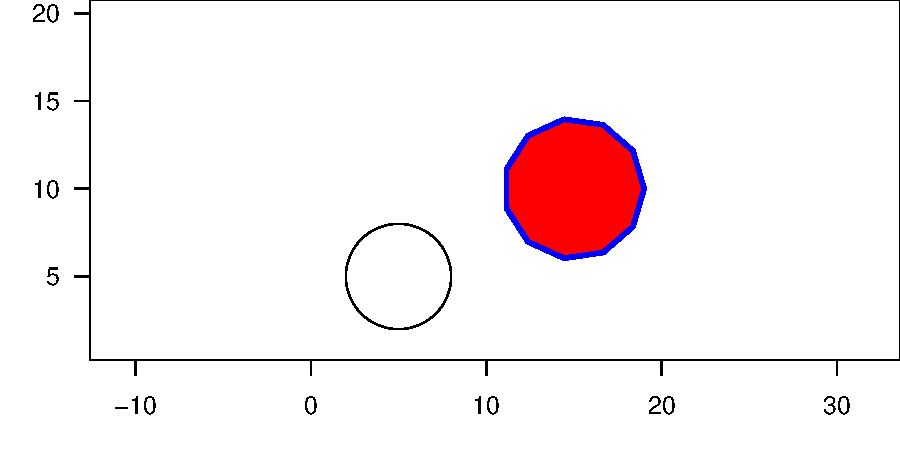
\includegraphics[width=\textwidth]{./fig/exfunsolb-1} 

}



\end{knitrout}
\end{frame}

%------------------------------------------------------------%

\begin{frame}[fragile]{Solution for exercise \arabic{exercisecount} III: functions}
\begin{knitrout}\scriptsize
\definecolor{shadecolor}{rgb}{0.961, 0.961, 0.961}\color{fgcolor}\begin{kframe}
\begin{alltt}
\hlcom{# can not be vectorized:}
\hlstd{x} \hlkwb{<-} \hlkwd{sample}\hlstd{(}\hlnum{1}\hlopt{:}\hlnum{20}\hlstd{,} \hlnum{15}\hlstd{) ;  y} \hlkwb{<-} \hlkwd{sample}\hlstd{(}\hlnum{1}\hlopt{:}\hlnum{20}\hlstd{,} \hlnum{15}\hlstd{) ; r} \hlkwb{<-} \hlkwd{runif}\hlstd{(}\hlnum{20}\hlstd{)}\hlopt{*}\hlnum{4}
\hlkwd{circle}\hlstd{(x,y,r,} \hlkwc{col}\hlstd{=}\hlkwd{rgb}\hlstd{(}\hlnum{1}\hlstd{,}\hlnum{0.5}\hlstd{,}\hlnum{0}\hlstd{,}\hlkwc{alpha}\hlstd{=}\hlnum{0.4}\hlstd{),} \hlkwc{border}\hlstd{=}\hlnum{NA}\hlstd{)}
\end{alltt}


{\ttfamily\noindent\color{warningcolor}{\#\# Warning in circle(x, y, r, col = rgb(1, 0.5, 0, alpha = 0.4), border = NA): Only the first element of the vectors is used.}}\begin{alltt}
\hlkwa{for}\hlstd{(i} \hlkwa{in} \hlnum{1}\hlopt{:}\hlnum{15}\hlstd{)} \hlkwd{circle}\hlstd{(x[i],y[i],r[i],} \hlkwc{col}\hlstd{=}\hlkwd{rgb}\hlstd{(}\hlnum{1}\hlstd{,}\hlnum{0.5}\hlstd{,}\hlnum{0}\hlstd{,}\hlkwc{alpha}\hlstd{=}\hlnum{0.4}\hlstd{),} \hlkwc{border}\hlstd{=}\hlnum{NA}\hlstd{)}
\end{alltt}
\end{kframe}

{\centering 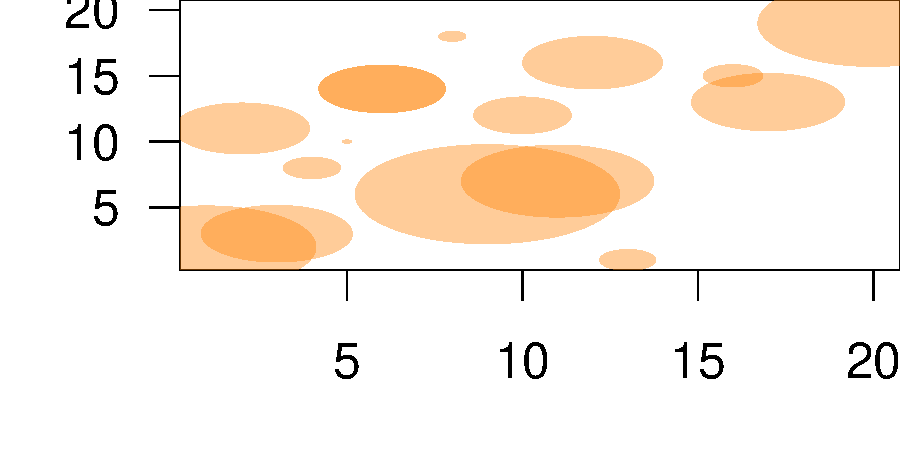
\includegraphics[width=0.4\textwidth]{./fig/exfunsolc-1} 

}



\end{knitrout}
\end{frame}

% ---------------------------

\section{Debugging}

% ---------------------------

\begin{frame}[fragile]{Debugging}
\begin{itemize}[<+->]
\item Your code throws an error.
You didn't call the mentioned function.
Obviously, your code calls some function calling some function calling some function calling [you get the idea] which in the end creates an error.
To trace back this path, you can use \rcode{traceback()}.

\item Now that you know where the error originates from, you set \rcode{options(error=recover)}.
You run your code again, but this time R waits at the level creating an error.
You examine the environment within the function, play around with the objects and internal function code, until the bug has been fixed.
You have just debugged a function.

\item You want to step into the function you are developing at a specific point.
You add \rcode{browser()} at that point of the code.
\end{itemize}
\end{frame}

% ---------------------------

\begin{frame}[fragile]{Debugging: useful functions + Resources}
\begin{tabular}{ll}
\pause source("projectFuns.R") & execute complete file\\
\pause traceback() & find error source in sequence of function calls\\
\pause options(warn=2) & warnings to error. default 0\\
\pause browser() & go into function environment: \rcode{n}, \rcode{s}, \rcode{f}, \rcode{c}, \rcode{Q}\\
\pause \alert{options(error=recover)} & \alert{open interactive session where error occurred}\\
\pause debug(funct) & toggle linewise function execution\\
\pause undebug(funct) & after calling and fixing funct\\
\end{tabular}\\

\pause \vspace{1em}
\href{http://www.biostat.jhsph.edu/~rpeng/docs/R-debug-tools.pdf}{R. Peng (2002): Interactive Debugging Tools in R}\\
\href{https://www.stats.umanitoba.ca/files/statsweb/2011/03/debugging.pdf}{D. Murdoch (2010): Debugging in R}\\
\href{http://adv-r.had.co.nz/Exceptions-Debugging.html}{H. Wickham (2015): Advanced R: debugging}\\
Example: \href{https://www.r-bloggers.com/tracking-down-errors-in-r/}{Pete Werner Blog Post (2013)}
\end{frame}

%------------------------------------------------------------%

\begin{frame}[fragile]{Practice debugging, \datalinkText{lsc\_functions.R}}
\begin{exercise}{Debugging}
\begin{enumerate}
\item Load your package and the datasets. Correct the functions until\\
\rcode{lsc(calib\$P, calib\$Q, area=1.6)} returns the result below.
\item BONUS: commit each change to git.
\end{enumerate}
\end{exercise}

\begin{knitrout}
\definecolor{shadecolor}{rgb}{0.961, 0.961, 0.961}\color{fgcolor}

{\centering 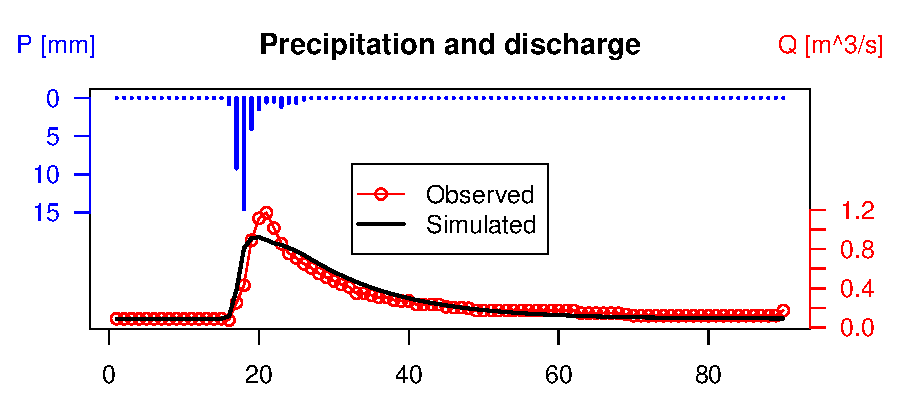
\includegraphics[width=\textwidth]{./fig/PQ_lsc-1} 

}



\end{knitrout}
\end{frame}

%------------------------------------------------------------%

\begin{frame}[fragile]{Solution for exercise \arabic{exercisecount}: Debugging}
\begin{itemize}
\item \rcode{stupid error you can easily remove} - traceback - find location of error - lsc\#73 - just comment it out
\item \rcode{harder to find but still stupid} - traceback - nse\#11 - ditto
\item \rcode{Error in plot: need finite 'ylim' value} - browser/options(error=recover) - lsc\#105 - NAs in Q - range(Q, na.rm=TRUE) - also in other applicable locations
\item \rcode{There were 50 or more warnings} - come from rmse being called in optimization - add argument quietNA (or similar) to lsc that is passed to rmse in lsc\#79
\end{itemize}
\end{frame}

%------------------------------------------------------------%
%------------------------------------------------------------%
\end{document}
%------------------------------------------------------------%
%------------------------------------------------------------%

